\chapter{模型/视图 编程}

\section{模型/视图编程简介} 

Qt 中包含了一系列的项目视图类,他们使用了模型/视图架构来管理数据和显示之间的关系。此架构的功能分离特征给开发人员在自定义项目的呈现形式时带来了很大的灵活性,并提供标准的模型接口,以允许将各种数据源与现有项目视图一起使用。在本文档中,我们对模型/视图进行了简要介绍,概述了所涉及的概念,并描述了项目视图系统的结构特征。介绍了体系结构中的每个组件,并给出了示例,这些示例告诉我们如何使用所提供的类。

\section{模型/视图体系架构}

模型-视图-控制器(MVC)是源自 Smalltalk 的设计模式,在构建用户界面时经常使用。在《设计模式》一书中,Gamma 等人写到:

\begin{quote}
MVC 由三种对象组成。模型是应用程序对象,视图是其在屏幕上的呈现,控制器定义了用户界面对用户输入的反应方式。 在MVC之前,用户界面设计往往会将这些对象整合在一起。 MVC 使它们解耦以增加灵活性和重用性。	
\end{quote}

如果将视图和控制器对象组合在一起,就是模型/视图架构。基于将数据的存储方式与向用户呈现的方式分开的原理,模型/视图架构提供了一个更简单的框架。这种分离使得可以在几个不同的视图中显示相同的数据,并实现新的视图类型,而无需更改基础数据结构。为了灵活处理用户输入,我们引入了委托的概念。在此框架中使用委托的好处在于,它允许自定义呈现和编辑数据项的方式。

\begin{tabular}{|l|m{25em}|}
\hline
    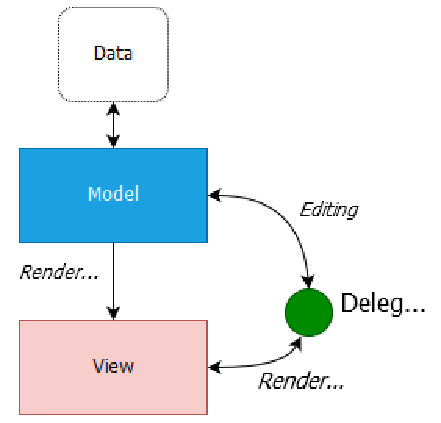
\includegraphics[width=0.5\textwidth]{Model_View_architecture.pdf}
  & 模型/视图架构 模型与数据源通信,为架构中的其他组件提供接口。通信的性质取决于数据源的类型以及模型的实现方式。

视图从模型中获取模型索引; 这些索引是对数据项的引用。 通过向模型提供模型索引,视图可以从数据源检索出数据项。

在标准视图中,委托负责渲染显示数据项。 当编辑项目后,委托将直接通过模型索引与模型进行通信。\\

\hline	
\end{tabular}

通常,模型/视图类可以分为上述三个组:模型,视图和委托。这些组件中的每个组件都由抽象类定义,这些抽象类提供了公共接口,并在某些情况下提供了一些功能的默认实现。抽象类应被子类化,以提供其他组件期望的全部功能;当然也可以编写专用组件。

模型、视图和委托之间通过信号槽通信。

\begin{itemize}
\item 数据源的数据发生改变时模型将发射信号通知视图。
\item 用户交互发生改变时,视图将发射相应的信号。
\item 在编辑期间,委托将发射信号来告知模型和视图有关编辑器的状态。
\end{itemize}

\section{模型}

所有项目模型均基于 QAbstractItemModel 类。此类定义一个接口,视图和委托使用该接口访问数据。数据本身不必存储在模型中。它可以保存在由单独的类,文件,数据库或某些其他应用程序组件提供的数据结构或存储库中。

有关模型的基本概念在 “模型类”部分中介绍。

QAbstractItemModel 提供了一个数据接口,该接口足够灵活,可以处理以表,列表和树的形式表示数据的视图。但是,当为列表和类似表的数据结构实现新模型时,QAbstractListModel 和 QAbstractTableModel 类是更好的选择,因为它们提供了常用功能的默认实现。这些类中的每一个都可以被子类化以提供支持特殊类型的列表和表的模型。

在 创建新模型 部分中讨论了模型子类化的过程。

Qt提供了一些现成的模型,可用于处理数据项:

\begin{itemize}
\item QStringListModel 用于存储一列简单的 QString 类型的项目。
\item QStandardItemModel 用于管理更复杂的树形结构项目,每个项目可以包含任意数据。
\item QFileSystemModel 提供有关本地归档系统中文件和目录的信息。
\item QSqlQueryModel,QSqlTableModel 和 QSqlRelationalTableModel 用于在使用模型/视图架构时访问数据库。
\end{itemize}

如果这些标准模型不满足您的要求,则可以将 QAbstractItemModel,QAbstractListModel 或 QAbstractTableModel 子类化以创建您自己的自定义模型。

\section{视图}

Qt 提供了针对各种视图的完整实现:QListView 用于显示项目列表,QTableView 用于显示表结构模型的数据,QTreeView 在一个分层次的结构列表中显示数据项。这些类均基于 QAbstractItemView 抽象基类。尽管这些类都是已经实现好的,但也可以将它们子类化以提供满足我们需求的自定义视图。

所有可用的视图可在 视图类 部分中进行查阅。
